\documentclass[journal,onecolumn]{IEEEtran}

% * CITATION PACKAGES *
\usepackage{cite}

% * GRAPHICS RELATED PACKAGES *
\usepackage{graphicx}
\graphicspath{{./}{../}{./Week9 work/}{./output_final/}}
\DeclareGraphicsExtensions{.pdf,.jpeg,.jpg,.png}

% * MATH PACKAGES *
\usepackage{amsmath}
\usepackage{amssymb}
\usepackage{amsfonts}
\usepackage{bm}

% * ALIGNMENT PACKAGES *
\usepackage{array}

% * PDF, URL AND HYPERLINK PACKAGES *
\usepackage{url}
\usepackage{booktabs}
\usepackage{microtype}
\usepackage[hidelinks]{hyperref}
\usepackage{float}

% Correct bad hyphenation here
\hyphenation{op-tical net-works semi-conduc-tor}

\begin{document}

% Paper title
\title{Semantic-Aware Integrated Sensing and Communication (ISAC) Networks with Power-Domain NOMA and 3D Elevation-Dependent Path Loss under Uncertain Eavesdropper Locations}

% Author names and affiliations
\author{
Dr. Sunandita Debnath, Dr. Gaurav Kr. Pandey,
Nikhil~Gadige,
Anuj~Saha,
Divyanshu~Ghosh,
Mohli~Thapa%
\thanks{N. Gadige, A. Saha, D. Ghosh, and M. Thapa are with the Department of Computer Science and Engineering, Indian Institute of Information Technology Vadodara, under the Summer Research Program 2026.}%
\thanks{E-mails: 202351037@iiitvadodara.ac.in, 202351010@iiitvadodara.ac.in, 202351036@iiitvadodara.ac.in, 202351084@iiitvadodara.ac.in.}
}

% Make the title area
\maketitle

\begin{abstract}
Integrated Sensing and Communication (ISAC) has emerged as a key technology for 6G wireless systems to share spectrum and hardware resources efficiently. However, resource scarcity and security vulnerability in Air-to-Ground (A2G) networks pose critical implementation challenges. In this report, we present the design and system model of a Semantic-Aware ISAC Network assisted by an aerial Reconfigurable Intelligent Surface (RIS) mounted on an Unmanned Aerial Vehicle (UAV) ($R$). To optimize spectral efficiency, we employ Power-Domain Non-Orthogonal Multiple Access (PD-NOMA) to serve a near user (Target $T$) and a distant mobile user ($U$) simultaneously. Crucially, all communications and sensing nodes operate under semantic-aware metrics, shifting the focus from error-free bit transmission to the preservation of meaning. The network is subjected to eavesdropping from terrestrial nodes ($E_1, \dots, E_{K_e}$) whose physical locations are imperfectly known (uncertain locations). Additionally, the system is subjected to directional jamming from a UAV Jammer ($J$), which also performs monostatic radar sensing. We formulate the detailed mathematical models, signal flows, and multi-stage beamforming (analog and digital) for the entire network. To resolve the joint optimization problem, we evaluate the convergence and utility of five reinforcement learning algorithms: Random Walk, Single-Agent TD3PG (SATD3PG), Single-Agent SAC (SASAC), Multi-Agent TD3PG (MATD3PG), and Multi-Agent PPO (MAPPO), under a combined utility function that balances physical layer security, sensing probability, and Cram\'{e}r-Rao Bound (CRB) feasibility constraints.
\end{abstract}

\begin{IEEEkeywords}
Integrated Sensing and Communication (ISAC), Semantic Communications, Power-Domain NOMA, Reconfigurable Intelligent Surface (RIS), Location Uncertainty, Digital and Analog Beamforming, Deep Reinforcement Learning.
\end{IEEEkeywords}

\IEEEpeerreviewmaketitle

\section{Introduction}
Future 6G networks are envisioned to go beyond traditional communication by integrating radar sensing and semantic intelligence into a unified architecture. Integrated Sensing and Communication (ISAC) allows wireless nodes to simultaneously transmit information and sense environment parameters (e.g., target localization and tracking) using the same frequency bands and hardware.

To overcome severe blockages and path loss in urban environments, Reconfigurable Intelligent Surfaces (RIS) mounted on Unmanned Aerial Vehicles (UAVs) ($R$) can be deployed as passive aerial reflectors. By adjusting the phase shifts of the RIS elements, a virtual Line-of-Sight (LoS) link can be established between a terrestrial Base Station (BS) $B$ and ground users, dramatically increasing signal coverage and physical layer security.

In parallel, semantic communications represent a paradigm shift from Shannon's classical information theory, which focuses solely on the accurate transmission of bit sequences. Rather than guaranteeing bit-level fidelity, a semantic-aware transmitter extracts the task-relevant meaning of a message through a learned semantic encoder and conveys only a compact set of semantic symbols that are sufficient for the intended receiver to reconstruct that meaning. This approach drastically reduces the required channel symbols and increases resilience against severe fading and interference, while simultaneously offering an inherent security advantage: an intercepted semantic symbol stream is largely uninterpretable to any node that does not possess the same semantic encoder-decoder pair, since meaning recovery -- unlike bit recovery -- depends on shared semantic knowledge rather than on the raw symbols themselves.

In this work, we consider a location-uncertainty eavesdropper model to ensure robust physical layer security. Eavesdroppers are located at positions that are estimated by legitimate nodes with a bounded error. The location of the $e$-th eavesdropper is represented as $\mathbf{p}_{E_e} = \widetilde{\mathbf{p}}_{E_e} + \Delta\mathbf{p}_{E_e}$, where $\widetilde{\mathbf{p}}_{E_e}$ is the estimated location and $\Delta\mathbf{p}_{E_e}$ is the estimation error bounded within a sphere of radius $\Delta Q_e$. We formulate the worst-case secrecy rates under this uncertainty.

This report outlines the implementation details and mathematical models. We design a semantic-aware ISAC network incorporating:
\begin{enumerate}
    \item \textbf{Elevation-Dependent Path Loss}: Incorporating 3D elevation angle $\theta_{ij}$, elevation-dependent LoS probability $P_{\text{LoS}}(\theta_{ij})$, and elevation-dependent Rician fading.
    \item \textbf{Digital and Analog Beamforming}: Steering the downlink signals via digital beamforming at the BS, passive analog phase-shift beamforming at the RIS, and multi-antenna digital jamming beamforming at the UAV Jammer.
    \item \textbf{Power-Domain NOMA (PD-NOMA)}: Serving a near Target user ($T$) and a distant Mobile User ($U$) over a superposed downlink signal, using semantic-aware Successive Interference Cancellation (SIC), in which the near user first reconstructs the far user's semantic information and removes its contribution before decoding its own semantic symbols.
    \item \textbf{Semantic Performance Metrics}: Characterizing semantic similarity, semantic rate, and semantic distortion for all links based on a trained DeepSC lookup table (linear interpolation), governed by the semantic compression ratio $M/K$, where we explicitly define $M=10$ and $K=15$.
\end{enumerate}

\begin{figure}[H]
    \centering
    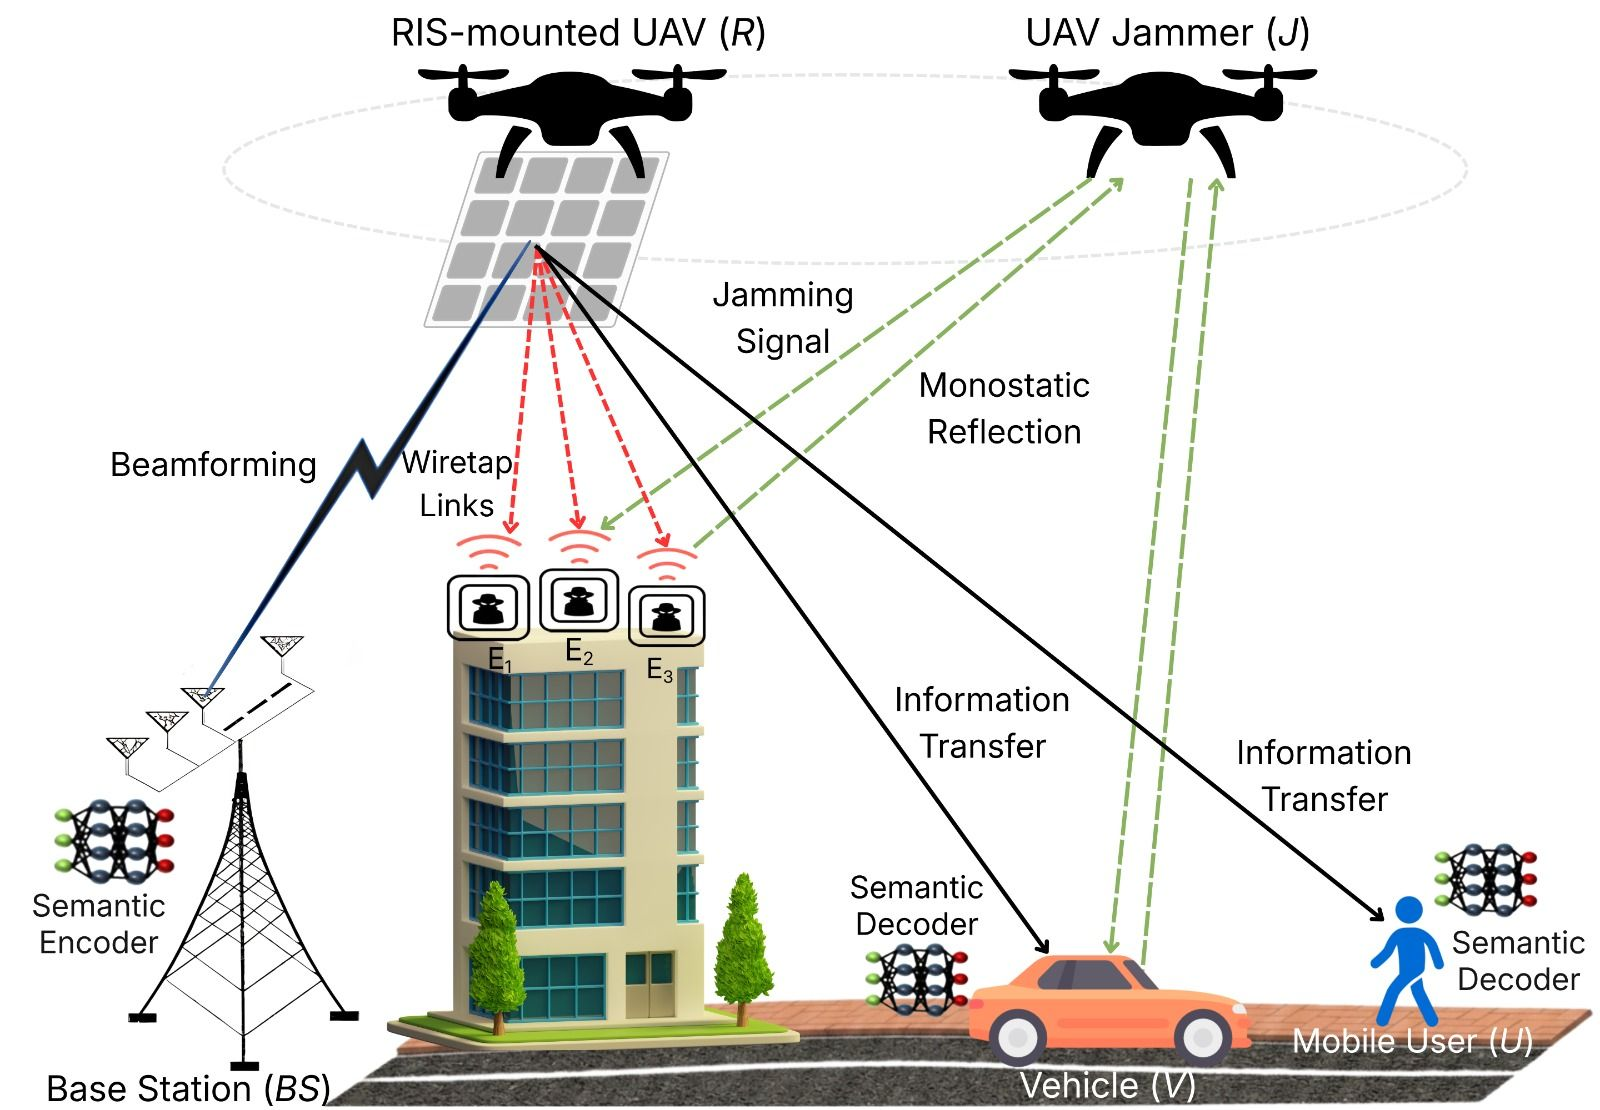
\includegraphics[width=0.65\textwidth]{system-model.jpeg}
    \caption{System model of the proposed semantic-aware RIS-assisted UAV ISAC network.}
    \label{fig:system_model}
\end{figure}

\section{System Architecture and Node Descriptions}
We consider an aerial-terrestrial co-existing network operating in a bounded 3D space. The system consists of the following key nodes:
\begin{itemize}
    \item \textbf{Base Station ($B$)}: Located at $\mathbf{p}_B = [x_B, y_B, z_B]^T$. It acts as a semantic-aware transmitter equipped with $N_B$ antennas, sending superposed downlink signals to paired users.
    \item \textbf{RIS-mounted UAV ($R$)}: An aerial platform hovering at $\mathbf{p}_R = [x_R, y_R, z_R]^T$, equipped with $N_R$ passive reflecting elements to establish cascaded communication paths.
    \item \textbf{UAV Jammer ($J$)}: An adversarial aerial node located at $\mathbf{p}_J = [x_J, y_J, z_J]^T$, equipped with $N_J$ antennas. It transmits directional jamming signals to degrade eavesdropper rates while performing monostatic radar sensing reflections.
    \item \textbf{Target ($T$)}: A near user and active communicator located at $\mathbf{p}_T = [x_T, y_T, z_T]^T$. In the downlink, it decodes the NOMA signal using semantic-aware SIC. In the uplink, it transmits semantic messages to the Base Station $B$ (via the RIS $R$) and directly to the Mobile User $U$ via V2X.
    \item \textbf{Mobile User ($U$)}: A distant user located at $\mathbf{p}_U = [x_U, y_U, z_U]^T$, decoding the downlink far-user signal directly.
    \item \textbf{Eavesdroppers ($E_1, \dots, E_{K_e}$)}: Passive ground nodes trying to intercept downlink semantic transmissions. Their positions are estimated with uncertainty. For the $e$-th eavesdropper ($e \in \{1, \dots, K_e\}$), the location is modeled as:
    \begin{equation}
        \mathbf{p}_{E_e} = \widetilde{\mathbf{p}}_{E_e} + \Delta\mathbf{p}_{E_e} = \begin{bmatrix} \tilde{x}_{E_e} + \Delta x_e \\ \tilde{y}_{E_e} + \Delta y_e \\ \tilde{z}_{E_e} + \Delta z_e \end{bmatrix},
    \end{equation}
    where $\widetilde{\mathbf{p}}_{E_e} = [\tilde{x}_{E_e}, \tilde{y}_{E_e}, \tilde{z}_{E_e}]^T$ is the estimated location, and the error vector $\Delta\mathbf{p}_{E_e}$ is bounded within a sphere:
    \begin{equation}
        \|\Delta\mathbf{p}_{E_e}\|_2 = \sqrt{\Delta x_e^2 + \Delta y_e^2 + \Delta z_e^2} \le \Delta Q_e.
    \end{equation}
    We assume the eavesdroppers lie on the ground ($\tilde{z}_{E_e} = 0, \Delta z_e = 0$), so the uncertainty sphere reduces to a 2D circle on the horizontal plane. A practical and feasible uncertainty radius of $\Delta Q_e = 15.0\text{ m}$ is chosen, reflecting standard localization errors. In our evaluations, we consider $K_e = 3$ eavesdroppers ($E_1, E_2, E_3$).
\end{itemize}

\section{Mathematical Formulations}

\subsection{Elevation-Dependent Air-to-Ground Path Loss and Channel Model}
For any propagation link $ij$ between a transmitter $i$ at position $\mathbf{p}_i = [x_i, y_i, z_i]^T$ and a receiver $j$ at $\mathbf{p}_j = [x_j, y_j, z_j]^T$, the 3D Euclidean distance is:
\begin{equation}
    d_{ij} = \|\mathbf{p}_i - \mathbf{p}_j\|_2 = \sqrt{(x_i - x_j)^2 + (y_i - y_j)^2 + (z_i - z_j)^2}.
\end{equation}
The 2D horizontal distance is $d_{\text{2D}, ij} = \sqrt{(x_i - x_j)^2 + (y_i - y_j)^2}$. The vertical elevation difference is $\Delta z_{ij} = |z_i - z_j|$. The 3D elevation angle $\theta_{ij}$ (in degrees) is given by:
\begin{equation}
    \theta_{ij} = \arcsin\left( \frac{\Delta z_{ij}}{d_{ij}} \right) \cdot \frac{180}{\pi}.
\end{equation}
Due to the variations in building heights, blockages, and terrain, the probability of establishing a Line-of-Sight (LoS) link is modeled as a logistic-type function of the elevation angle $\theta_{ij}$:
\begin{equation}
    P_{\text{LoS}}(\theta_{ij}) = \frac{1}{1 + a \cdot \exp\left( -b (\theta_{ij} - a) \right)},
\end{equation}
where $a$ and $b$ are calibration constants representing the urban environment (e.g., $a = 9.61, b = 0.16$ for typical urban environments). The Non-Line-of-Sight (NLoS) probability is $P_{\text{NLoS}}(\theta_{ij}) = 1 - P_{\text{LoS}}(\theta_{ij})$.

The path losses for the LoS and NLoS states, incorporating excessive attenuation, are modeled as:
\begin{equation}
    \text{PL}_{\text{LoS}}(d_{ij}) = 20\log_{10}\left( \frac{4\pi d_{ij} f_c}{c} \right) + \eta_{\text{LoS}},
\end{equation}
\begin{equation}
    \text{PL}_{\text{NLoS}}(d_{ij}) = 20\log_{10}\left( \frac{4\pi d_{ij} f_c}{c} \right) + \eta_{\text{NLoS}},
\end{equation}
where $f_c$ is the carrier frequency, $c$ is the speed of light, and $\eta_{\text{LoS}}$, $\eta_{\text{NLoS}}$ represent the excessive path loss factors in dB for LoS and NLoS links, respectively. The mean path loss in dB is:
\begin{equation}
    \overline{\text{PL}}(d_{ij}, \theta_{ij}) = P_{\text{LoS}}(\theta_{ij}) \cdot \text{PL}_{\text{LoS}}(d_{ij}) + \left(1 - P_{\text{LoS}}(\theta_{ij})\right) \cdot \text{PL}_{\text{NLoS}}(d_{ij}).
\end{equation}
Converting this to linear gain yields:
\begin{equation}
    \text{PL}_{\text{linear}}(d_{ij}, \theta_{ij}) = 10^{-\overline{\text{PL}}(d_{ij}, \theta_{ij}) / 10}.
\end{equation}

For Rician fading, the small-scale fading channel is modeled as:
\begin{equation}
    \mathbf{h}_{ij} = \sqrt{\frac{K}{K+1}} \bar{\mathbf{h}}_{ij} + \sqrt{\frac{1}{K+1}} \tilde{\mathbf{h}}_{ij},
\end{equation}
where $\bar{\mathbf{h}}_{ij}$ is the deterministic LoS component, $\tilde{\mathbf{h}}_{ij} \sim \mathcal{CN}(0, \mathbf{I})$ is the scattered NLoS component, and $K$ is the Rician $K$-factor scaling with the elevation angle:
\begin{equation}
    K_{\text{dB}}(\theta_{ij}) = K_0 + \alpha_K \theta_{ij}, \quad K(\theta_{ij}) = 10^{K_{\text{dB}}(\theta_{ij}) / 10},
\end{equation}
where $K_0 = 3.0$ dB and $\alpha_K = 0.15$ dB/degree. The final channel power gain is:
\begin{equation}
    g_{ij} = \text{PL}_{\text{linear}}(d_{ij}, \theta_{ij}) \cdot |\mathbf{h}_{ij}|^2.
\end{equation}

\subsection{Multi-Stage Digital and Analog Beamforming}
In our network, beamforming occurs at three stages: digital beamforming at the BS, analog reflection beamforming at the RIS, and digital beamforming at the UAV Jammer.

\subsubsection{Base Station (BS) Digital Beamforming}
The BS is equipped with $N_B$ antennas and performs digital beamforming. Let $\mathbf{w}_B \in \mathbb{C}^{N_B \times 1}$ be the digital beamforming vector satisfying the power constraint $\|\mathbf{w}_B\|_2 = 1$. The BS steers the superposed NOMA signal $s$ toward the RIS-mounted UAV $R$. Since digital beamforming operates in the baseband, it allows full control over both amplitude and phase.

\subsubsection{RIS Analog Reflection Beamforming}
The RIS consists of $N_R$ passive reflecting elements. It performs passive analog phase-only beamforming. The reflection coefficient matrix is defined as:
\begin{equation}
    \bm{\Phi} = \operatorname{diag}\left( e^{j\phi_1}, e^{j\phi_2}, \dots, e^{j\phi_{N_R}} \right) \in \mathbb{C}^{N_R \times N_R},
\end{equation}
where $\phi_n \in [0, 2\pi)$ is the phase shift of the $n$-th reflecting element. The RIS elements passively reflect the incident wave without amplification. The cascaded channel vector from the BS to receiver $k \in \{T, U\}$ via the RIS is:
\begin{equation}
    \mathbf{h}_{B,R,k} = \mathbf{h}_{R,k} \bm{\Phi} \mathbf{H}_{B,R} \in \mathbb{C}^{1 \times N_B},
\end{equation}
where $\mathbf{H}_{B,R} \in \mathbb{C}^{N_R \times N_B}$ is the channel matrix between the BS and RIS, and $\mathbf{h}_{R,k} \in \mathbb{C}^{1 \times N_R}$ is the channel vector from the RIS to receiver $k$. If the RIS phase shifts are adjusted to align constructively with the channel phases, the equivalent cascaded channel gain $g_{\text{cascaded}, k} = |\mathbf{h}_{B,R,k} \mathbf{w}_B|^2$ scales quadratically with $N_R$, yielding the simplified representation:
\begin{equation}
    g_{\text{cascaded}, k} = g_{B,R} \cdot g_{R,k} \cdot N_R^2,
\end{equation}
where $g_{B,R}$ and $g_{R,k}$ are the individual path-loss and fading gains of the BS-RIS and RIS-receiver links, respectively.

\subsubsection{UAV Jammer (J) Digital Beamforming}
The UAV Jammer $J$ is equipped with $N_J$ antennas and transmits artificial noise using a digital beamforming vector $\mathbf{w}_J \in \mathbb{C}^{N_J \times 1}$ with $\|\mathbf{w}_J\|_2 = 1$. The received jamming power gain at receiver $k$ is $g_{\text{jam}, k} = |\mathbf{h}_{J,k} \mathbf{w}_J|^2$, where $\mathbf{h}_{J,k} \in \mathbb{C}^{1 \times N_J}$ is the channel vector from the Jammer to receiver $k$. The Jammer can implement three alternative beamforming strategies:
\begin{enumerate}
    \item \textbf{Isotropic Beamforming}: Steers jamming power uniformly in all directions. The weight factor is:
    \begin{equation}
        \mathbf{w}_{\text{iso}} = \frac{1}{\sqrt{N_J}} \begin{bmatrix} e^{j\theta_1} & e^{j\theta_2} & \dots & e^{j\theta_{N_J}} \end{bmatrix}^T,
    \end{equation}
    where $\theta_n \sim \mathcal{U}(0, 2\pi)$ are independent random phases.
    \item \textbf{Maximum Ratio Transmission (MRT)}: Steers maximum jamming power directly toward a targeted eavesdropper $E_e$ with channel $\mathbf{h}_{J,E_e}$:
    \begin{equation}
        \mathbf{w}_{\text{mrt}} = \frac{\mathbf{h}_{J,E_e}^H}{\|\mathbf{h}_{J,E_e}\|_2}.
    \end{equation}
    \item \textbf{Null-Space (NS) Beamforming}: Projects the jamming signal into the null-space of the legitimate mobile user's channel $\mathbf{h}_{J,U}$, ensuring zero interference at the user while jamming the eavesdroppers. The weight factor is:
    \begin{equation}
        \mathbf{w}_{\text{ns}} = \frac{\mathbf{P} \mathbf{v}}{\|\mathbf{P} \mathbf{v}\|_2}, \quad \mathbf{P} = \mathbf{I}_{N_J} - \frac{\mathbf{h}_{J,U}^H \mathbf{h}_{J,U}}{\|\mathbf{h}_{J,U}\|_2^2},
    \end{equation}
    where $\mathbf{P}$ is the projection matrix, and $\mathbf{v} \in \mathbb{C}^{N_J \times 1}$ is a random vector.
\end{enumerate}

\subsubsection{Jammer Sensing Beamforming}
For radar target tracking, the Jammer uses dedicated sensing beamforming $\mathbf{w}_{\text{sense}}$ to focus the sensing power on the Target $T$ and the eavesdroppers $E_e$ using orthogonal waveforms, ensuring no mutual interference.

\subsection{Power-Domain NOMA and Successive Interference Cancellation}
The BS transmits a superposed signal to serve both the Target $T$ and the Mobile User $U$ over the same resource block:
\begin{equation}
    s = \sqrt{a_N P_B} s_N + \sqrt{a_F P_B} s_F,
\end{equation}
where $P_B$ is the BS transmit power, and $a_N, a_F$ are the NOMA power allocation factors satisfying $a_N + a_F = 1$ and $a_F > a_N \ge 0$. Legitimate receivers are ordered based on their effective channel gains. Under normal conditions, the Target $T$ is closer than Mobile User $U$, yielding $g_T \ge g_U$. The received jamming interference power at receiver $k \in \{T, U\}$ is:
\begin{equation}
    P_{J, k} = P_J \cdot g_{\text{jam}, k},
\end{equation}
where $P_J$ is the jammer transmit power, and $g_{\text{jam}, k}$ is the channel gain under the selected jammer beamforming strategy.

\subsubsection{Distant (Far) User Semantic Decoding}
The Mobile User $U$ decodes its signal $s_F$ directly by treating $s_N$ as noise. The received SINR at $U$ is:
\begin{equation}
    \gamma_F = \frac{a_F P_B g_U}{a_N P_B g_U + P_{J, U} + \sigma^2},
\end{equation}
where $\sigma^2$ is the thermal noise power. The resulting SINR feeds the semantic decoder to evaluate semantic similarity $S_U(\gamma_F)$ and rate $R_{\text{sem}, U}$.

\subsubsection{Near User Semantic-Aware SIC Decoding}
The Target $T$ first decodes the far user's signal $s_F$, reconstructs its contribution, and subtracts it before decoding its own signal $s_N$. Assuming perfect semantic-level SIC, the SINR for decoding $s_N$ at $T$ is:
\begin{equation}
    \gamma_N = \frac{a_N P_B g_T}{P_{J, T} + \sigma^2}.
\end{equation}
The target evaluates its semantic similarity $S_T(\gamma_N)$ and semantic rate $R_{\text{sem}, T}$ based on this SINR.

\subsection{Uplink and V2X Semantic Communications}
The Target $T$ also acts as an uplink transmitter using power $P_T$:
\begin{itemize}
    \item \textbf{Uplink V2I (Target to BS via RIS)}: The SINR at the BS is:
    \begin{equation}
        \gamma_{\text{uplink}} = \frac{P_T g_{T, R, B}}{P_{J, B} + \sigma^2},
    \end{equation}
    where $g_{T, R, B}$ is the cascaded Target-RIS-BS channel gain, and $P_{J, B} = P_J g_{J, B}$ is the jamming power received at the BS.
    \item \textbf{V2X Direct Semantic Link (Target to Mobile User U)}: The SINR at $U$ is:
    \begin{equation}
        \gamma_{\text{V2X}} = \frac{P_T g_{T, U}}{P_{J, U} + \sigma^2},
    \end{equation}
    where $g_{T, U}$ is the direct Target-User ground channel gain.
\end{itemize}

\subsection{Monostatic and Bistatic Radar Target Sensing and Selection Combining}
The Jammer $J$ performs radar sensing towards the Target $T$ and the eavesdroppers $E_e$. To maximize detection coverage, selection combining is employed between monostatic sensing (Jammer echo) and bistatic sensing (BS-to-target-to-Jammer):
\begin{align}
    \text{SNR}_{\text{radar}, T} &= \max\left( \text{SNR}_{\text{mono}, T},\, \text{SNR}_{\text{bi}, T} \right), \\
    \text{SNR}_{\text{radar}, E_e} &= \max\left( \text{SNR}_{\text{mono}, E_e},\, \text{SNR}_{\text{bi}, E_e} \right),
\end{align}
where the monostatic and bistatic sensing SNRs are given by:
\begin{equation}
    \text{SNR}_{\text{mono}, k} = \frac{P_{J, \text{sense}} \cdot g_{J,k}^2 \cdot G_p}{\sigma^2}, \quad
    \text{SNR}_{\text{bi}, k} = \frac{P_B \cdot g_{B, k} \cdot g_{J, k} \cdot G_p}{\sigma^2}, \quad k \in \{T, E_e\},
\end{equation}
with $G_p = 10^7$ being the radar processing gain. The sensing detection probabilities are evaluated via the empirical detection characteristic:
\begin{equation}
    P_{d, T} = \frac{1}{1 + \exp\left( -\kappa (\text{SNR}_{\text{radar}, T, \text{dB}} - \tau) \right)}, \quad
    P_{d, E_e} = \frac{1}{1 + \exp\left( -\kappa (\text{SNR}_{\text{radar}, E_e, \text{dB}} - \tau) \right)},
\end{equation}
where $\kappa = 0.4$ and $\tau = 2.0\text{ dB}$. The Cram\'{e}r-Rao Bound (CRB) for target tracking is:
\begin{equation}
    \text{CRB}_T = \frac{1}{\text{SNR}_{\text{radar}, T}}.
\end{equation}

\subsection{Eavesdropper Wiretap Model and Secrecy Rate Analysis}
To ensure robust security, the legitimate nodes assume the worst-case eavesdropping scenario. Under the location uncertainty model, the cascaded BS-RIS-Eavesdropper gain is maximized, while the Jammer-to-Eavesdropper gain is minimized. For the $e$-th eavesdropper $E_e$, the modified 2D distances are:
\begin{equation}
    d_{\text{2D}, RE_e}^{\text{modified}} = \max(d_{\text{2D}, RE_e} - \Delta Q_e, 0), \quad
    d_{\text{2D}, JE_e}^{\text{modified}} = d_{\text{2D}, JE_e} + \Delta Q_e.
\end{equation}
The maximized cascaded gain $g_{E_e}^{\max}$ and minimized jamming gain $g_{J, E_e}^{\min}$ are computed using these modified distances. The worst-case wiretap SINRs at eavesdropper $E_e$ are:
\begin{equation}
    \gamma_{E_e, U} = \frac{a_F P_B g_{E_e}^{\max}}{a_N P_B g_{E_e}^{\max} + P_J g_{J, E_e}^{\min} + \sigma^2}, \quad
    \gamma_{E_e, T} = \frac{a_N P_B g_{E_e}^{\max}}{P_J g_{J, E_e}^{\min} + \sigma^2}.
\end{equation}

Under non-colluding eavesdropping, the maximum intercepted semantic rate across all $K_e$ eavesdroppers is evaluated for each legitimate user:
\begin{equation}
    R_{\text{leak}, T} = \max_{e \in \{1, \dots, K_e\}} R_{\text{sem}, E_e, T}(\gamma_{E_e, T}), \quad
    R_{\text{leak}, U} = \max_{e \in \{1, \dots, K_e\}} R_{\text{sem}, E_e, U}(\gamma_{E_e, U}).
\end{equation}
The individual semantic secrecy rates for Target $T$ and Mobile User $U$ are therefore formulated as:
\begin{equation}
    R_{\text{sec}, T} = \left[ R_{\text{sem}, T}(\gamma_N) - \max_{e \in \{1, \dots, K_e\}} R_{\text{sem}, E_e, T}(\gamma_{E_e, T}) \right]^+,
\end{equation}
\begin{equation}
    R_{\text{sec}, U} = \left[ R_{\text{sem}, U}(\gamma_F) - \max_{e \in \{1, \dots, K_e\}} R_{\text{sem}, E_e, U}(\gamma_{E_e, U}) \right]^+,
\end{equation}
where $[x]^+ = \max(x, 0)$, and $R_{\text{sem}}(\cdot)$ is obtained via the DeepSC lookup table.

To combine the communication security across legitimate nodes, Selection Combining (SC) is applied between the Near User (Target $T$) and Far User (Mobile User $U$):
\begin{equation}
    R_{\text{sec}}^{\text{SC}} = \max\left( R_{\text{sec}, T},\, R_{\text{sec}, U} \right),
\end{equation}
alongside the cumulative sum secrecy rate metric $R_{\text{sec}}^{\text{sum}} = R_{\text{sec}, T} + R_{\text{sec}, U}$.

\subsection{Semantic Communication Metrics and DeepSC Lookup Table}
For all semantic links, the semantic similarity score $S(\gamma)$ is obtained by linear interpolation of a pre-trained DeepSC lookup table. The lookup table values are summarized in Table~\ref{tab:deepsc_lookup}.
We explicitly set the number of semantic concepts in a semantic unit to $M=10$, and the number of transmitted channel symbols to $K=15$, yielding a semantic compression ratio of $M/K = 2/3 \approx 0.67$.

The semantic transmission rate $R_{\text{sem}}$ (in suts/sec) and semantic distortion $D_{\text{sem}}$ are defined as:
\begin{equation}
    R_{\text{sem}} = B \cdot \left( \frac{M}{K} \right) \cdot S(\gamma) \cdot \log_2(1 + \gamma),
\end{equation}
\begin{equation}
    D_{\text{sem}} = 1 - S(\gamma),
\end{equation}
where $B$ is the bandwidth. Crucially, the similarity $S(\gamma)$ saturates to $0.95$ at high SINR and decays to $0.67$ at low SINR, following the empirical DeepSC evaluation.

\begin{table}[H]
    \centering
    \caption{DeepSC Lookup Table: SINR vs. Semantic Similarity and Word Accuracy ($M=10, K=15$).}
    \label{tab:deepsc_lookup}
    \begin{tabular}{ccc}
        \toprule
        $\gamma_{\text{dB}}$ (dB) & Semantic Similarity $S(\gamma)$ & Word Accuracy \\
        \midrule
        -20 & 0.6712 & 0.3945 \\
        -18 & 0.7171 & 0.4351 \\
        -16 & 0.7517 & 0.4549 \\
        -14 & 0.8021 & 0.4899 \\
        -12 & 0.8257 & 0.5261 \\
        -10 & 0.8638 & 0.5742 \\
        -8  & 0.8867 & 0.6012 \\
        -6  & 0.9103 & 0.6551 \\
        -4  & 0.9227 & 0.6830 \\
        -2  & 0.9316 & 0.6957 \\
        0   & 0.9398 & 0.7124 \\
        2   & 0.9443 & 0.7305 \\
        4   & 0.9456 & 0.7354 \\
        6   & 0.9462 & 0.7339 \\
        8   & 0.9490 & 0.7340 \\
        10  & 0.9499 & 0.7403 \\
        12  & 0.9504 & 0.7397 \\
        14  & 0.9508 & 0.7417 \\
        16  & 0.9508 & 0.7334 \\
        18  & 0.9508 & 0.7327 \\
        20  & 0.9507 & 0.7321 \\
        \bottomrule
    \end{tabular}
\end{table}

\section{Multi-Objective Joint Secrecy and Sensing Optimization Problem}
The optimization goal is to maximize a single shared episode-wise objective that combines communication security (ASSR) and radar sensing capability ($P_d$).

For an episode $e$ consisting of $T_{\text{total}}$ time steps, the average secrecy rate under Selection Combining (SC) is:
\begin{equation}
    R_{\text{sec}}^{(e)} = \frac{1}{T_{\text{total}}} \sum_{t=1}^{T_{\text{total}}} R_{\text{sec}}^{\text{SC}}(t).
\end{equation}
The Average System Secrecy Ratio ($\operatorname{ASSR}^{(e)}$) is scaled to the $[0, 1]$ interval using a running maximum reference secrecy rate $R_{\text{ref}}$:
\begin{equation}
    \operatorname{ASSR}^{(e)} = \operatorname{clip}\left( \frac{R_{\text{sec}}^{(e)}}{R_{\text{ref}}}, 0, 1 \right), \quad R_{\text{ref}} = \max_{j \in \{1, \dots, e\}} R_{\text{sec}}^{(j)}.
\end{equation}
The sensing detection probability metric $P_d^{(e)}$ combines target and eavesdropper detection probabilities:
\begin{equation}
    P_d^{(e)} = \lambda_{1,\text{sense}} P_{d, E}^{(e)} + \lambda_{2,\text{sense}} P_{d, T}^{(e)}, \quad \lambda_{1,\text{sense}} + \lambda_{2,\text{sense}} = 1,
\end{equation}
where $\lambda_{1,\text{sense}}$ and $\lambda_{2,\text{sense}}$ (default = 0.5) are the weights for eavesdropper and target detection, respectively, and the eavesdropper detection probability is averaged over the $K_e$ nodes:
\begin{equation}
    P_{d, E}^{(e)} = \frac{1}{K_e} \sum_{e=1}^{K_e} P_{d, E_e}^{(e)}.
\end{equation}
To enforce the target tracking accuracy, we introduce a feasibility indicator based on the target-side CRB threshold $\delta_{\text{CRB}} = 10^8$:
\begin{equation}
    \mathbb{I}_{\text{CRB}}^{(e)} =
    \begin{cases}
        1, & \text{if } \operatorname{CRB}_{T}^{(e)} \le \delta_{\text{CRB}}, \\
        0, & \text{otherwise.}
    \end{cases}
\end{equation}
The final constrained episode multi-objective utility is:
\begin{equation}
    U^{(e)} = \widehat{U}^{(e)} \cdot \mathbb{I}_{\text{CRB}}^{(e)} = \left( \lambda_1 \operatorname{ASSR}^{(e)} + \lambda_2 P_d^{(e)} \right) \mathbb{I}_{\text{CRB}}^{(e)},
\end{equation}
where $\lambda_1, \lambda_2 \ge 0$ ($\lambda_1 + \lambda_2 = 1$, default $\lambda_1 = \lambda_2 = 0.5$) govern the trade-off between physical layer semantic security and sensing performance.

\section{Deep Reinforcement Learning Algorithms and Formulations}
We evaluate five reinforcement learning paradigms to solve the optimization problem.

\subsection{Random Walk (Baseline)}
Actions for RIS-UAV step, Jammer-UAV step, and power allocations are sampled uniformly at random at each time step:
\begin{equation}
    a_{n,t} \sim \mathcal{U}(-1, 1).
\end{equation}

\subsection{Single-Agent TD3PG (SATD3PG)}
A single centralized agent outputs a 9-dimensional joint action vector containing the movements of both UAVs and the power allocation parameters. It uses the Twin Delayed Deep Deterministic Policy Gradient (TD3) algorithm.
\begin{itemize}
    \item \textbf{Bellman Equation and Twin Critics}: The twin critic networks $Q_{\phi_1}$ and $Q_{\phi_2}$ are updated by minimizing:
    \begin{equation}
        L(\phi_i) = \mathbb{E}\left[ \left( y_t - Q_{\phi_i}(s_t, a_t) \right)^2 \right], \quad i \in \{1, 2\},
    \end{equation}
    where the target value $y_t$ is computed using target policy smoothing:
    \begin{equation}
        y_t = r_t + \gamma \min_{i=1,2} Q_{\phi_i'}\left( s_{t+1}, \pi_{\theta'}(s_{t+1}) + \bm{\epsilon} \right), \quad \bm{\epsilon} \sim \operatorname{clip}(\mathcal{N}(0, \sigma^2), -c, c).
    \end{equation}
    \item \textbf{Deterministic Policy Gradient}: The actor network $\pi_{\theta}$ is updated using the deterministic policy gradient, delayed by a frequency $d$:
    \begin{equation}
        \nabla_{\theta} J(\theta) = \mathbb{E}\left[ \nabla_a Q_{\phi_1}(s, a)|_{a=\pi_\theta(s)} \nabla_{\theta} \pi_{\theta}(s) \right].
    \end{equation}
\end{itemize}

\subsection{Single-Agent Soft Actor-Critic (SASAC)}
A single agent outputs the joint action using Soft Actor-Critic (SAC) to maximize both the reward and policy entropy.
\begin{itemize}
    \item \textbf{Soft Q-Value Objective}: The twin Q-networks are updated by minimizing:
    \begin{equation}
        L(\phi_i) = \mathbb{E}\left[ \left( Q_{\phi_i}(s_t, a_t) - \left( r_t + \gamma \left( \min_{j=1,2} Q_{\phi_j'}(s_{t+1}, a_{t+1}) - \alpha_{\text{ent}} \log \pi_\theta(a_{t+1}|s_{t+1}) \right) \right) \right)^2 \right],
    \end{equation}
    where $a_{t+1} \sim \pi_{\theta}(\cdot|s_{t+1})$.
    \item \textbf{Stochastic Policy Update}: The actor policy is updated by minimizing:
    \begin{equation}
        J(\theta) = \mathbb{E}\left[ \alpha_{\text{ent}} \log \pi_{\theta}(a_t|s_t) - \min_{i=1,2} Q_{\phi_i}(s_t, a_t) \right],
    \end{equation}
    where $\alpha_{\text{ent}}$ is the temperature scale.
\end{itemize}

\subsection{Multi-Agent TD3PG (MATD3PG)}
The action space is split among three cooperative agents: $agent_1$ (RIS-UAV movement), $agent_2$ (Jammer-UAV movement), and $agent_3$ (power allocation), each with its own decentralized actor network $\pi_{\theta_n}$.
\begin{itemize}
    \item \textbf{Centralized Twin Critics}: Take the global state $s$ and the joint action $\mathbf{a} = [a_1, a_2, a_3]$. The Q-networks are updated using the joint actions:
    \begin{equation}
        y_t = r_t + \gamma \min_{i=1,2} Q_{\phi_i'}\left( s_{t+1}, \pi_{\theta_1'}(s_{t+1}) + \bm{\epsilon}_1, \pi_{\theta_2'}(s_{t+1}) + \bm{\epsilon}_2, \pi_{\theta_3'}(s_{t+1}) + \bm{\epsilon}_3 \right).
    \end{equation}
    \item \textbf{Decentralized Actor Updates}: Each actor is updated using the centralized critic gradient:
    \begin{equation}
        \nabla_{\theta_n} J(\theta_n) = \mathbb{E}\left[ \nabla_{a_n} Q_{\phi_1}(s, a_1, a_2, a_3)|_{a_n=\pi_{\theta_n}(s)} \nabla_{\theta_n} \pi_{\theta_n}(s) \right].
    \end{equation}
\end{itemize}

\subsection{Multi-Agent Proximal Policy Optimization (MAPPO)}
Three decentralized stochastic policy actors $\pi_{\theta_n}$ are trained alongside a centralized value network $V_\psi(s)$.
\begin{itemize}
    \item \textbf{Clipped PPO Objective}: The policy networks are updated by maximizing the clipped surrogate objective:
    \begin{equation}
        L^{\text{CLIP}}(\theta_n) = \mathbb{E}\left[ \min\left( r_{t,n}(\theta_n) \widehat{A}_t, \operatorname{clip}\left( r_{t,n}(\theta_n), 1-\epsilon, 1+\epsilon \right) \widehat{A}_t \right) \right] + \beta_{\text{ent}} \mathcal{H}\left( \pi_{\theta_n}(\cdot|s_t) \right),
    \end{equation}
    where $r_{t,n}(\theta_n) = \frac{\pi_{\theta_n}(a_{n,t}|s_t)}{\pi_{\theta_n}^{\text{old}}(a_{n,t}|s_t)}$, $\mathcal{H}$ is the entropy, and $\widehat{A}_t$ is the Generalized Advantage Estimate (GAE) computed using the centralized value function $V_\psi(s)$:
    \begin{equation}
        \widehat{A}_t = \sum_{l=0}^{T-t-1} (\gamma \lambda_{\text{GAE}})^l \delta_{t+l}^V, \quad \delta_t^V = r_t + \gamma V_\psi(s_{t+1}) - V_\psi(s_t).
    \end{equation}
    \item \textbf{Centralized Value Update}: The value network $V_\psi$ is updated by minimizing:
    \begin{equation}
        L(\psi) = \mathbb{E}\left[ \left( V_\psi(s_t) - G_t \right)^2 \right],
    \end{equation}
    where $G_t$ is the discounted return.
\end{itemize}

\subsection{Hyperparameter Settings}
The complete hyperparameter settings for all five algorithms are summarized in Table~\ref{tab:hyperparameters}.

\begin{table}[H]
    \centering
    \caption{RL Training Hyperparameters.}
    \label{tab:hyperparameters}
    \begin{tabular}{lcccc}
        \toprule
        Hyperparameter & MAPPO & MATD3PG & SASAC & SATD3PG \\
        \midrule
        Number of Episodes & 8000 & 8000 & 8000 & 8000 \\
        Steps per Episode & 50 & 50 & 50 & 50 \\
        Batch Size & 64 & 64 & 64 & 64 \\
        Discount Factor $\gamma$ & 0.95 & 0.95 & 0.95 & 0.95 \\
        Soft Update $\tau$ & -- & 0.01 & 0.01 & 0.01 \\
        Replay Buffer Size & -- & 50000 & 50000 & 50000 \\
        Actor Learning Rate & $2.5 \times 10^{-4}$ & $3.0 \times 10^{-4}$ & $3.0 \times 10^{-4}$ & $3.0 \times 10^{-4}$ \\
        Critic Learning Rate & $2.5 \times 10^{-4}$ & $3.0 \times 10^{-4}$ & $3.0 \times 10^{-4}$ & $3.0 \times 10^{-4}$ \\
        Policy Noise & -- & 0.2 & -- & 0.2 \\
        Noise Clip $c$ & -- & 0.5 & -- & 0.5 \\
        Policy Update Freq $d$ & -- & 2 & -- & 2 \\
        Entropy Coefficient $\beta_{\text{ent}}$ & 0.01 & -- & 0.2 (fixed $\alpha_{\text{ent}}$) & -- \\
        GAE Parameter $\lambda_{\text{GAE}}$ & 0.95 & -- & -- & -- \\
        PPO Clip Parameter $\epsilon$ & 0.2 & -- & -- & -- \\
        Gradient Clipping Norm & 0.5 & -- & -- & -- \\
        Network Hidden Layers & 2 (64 units) & 2 (64 units) & 2 (64 units) & 2 (64 units) \\
        Activation Function & ReLU & ReLU & ReLU & ReLU \\
        \bottomrule
    \end{tabular}
\end{table}

\begin{figure}[H]
    \centering
    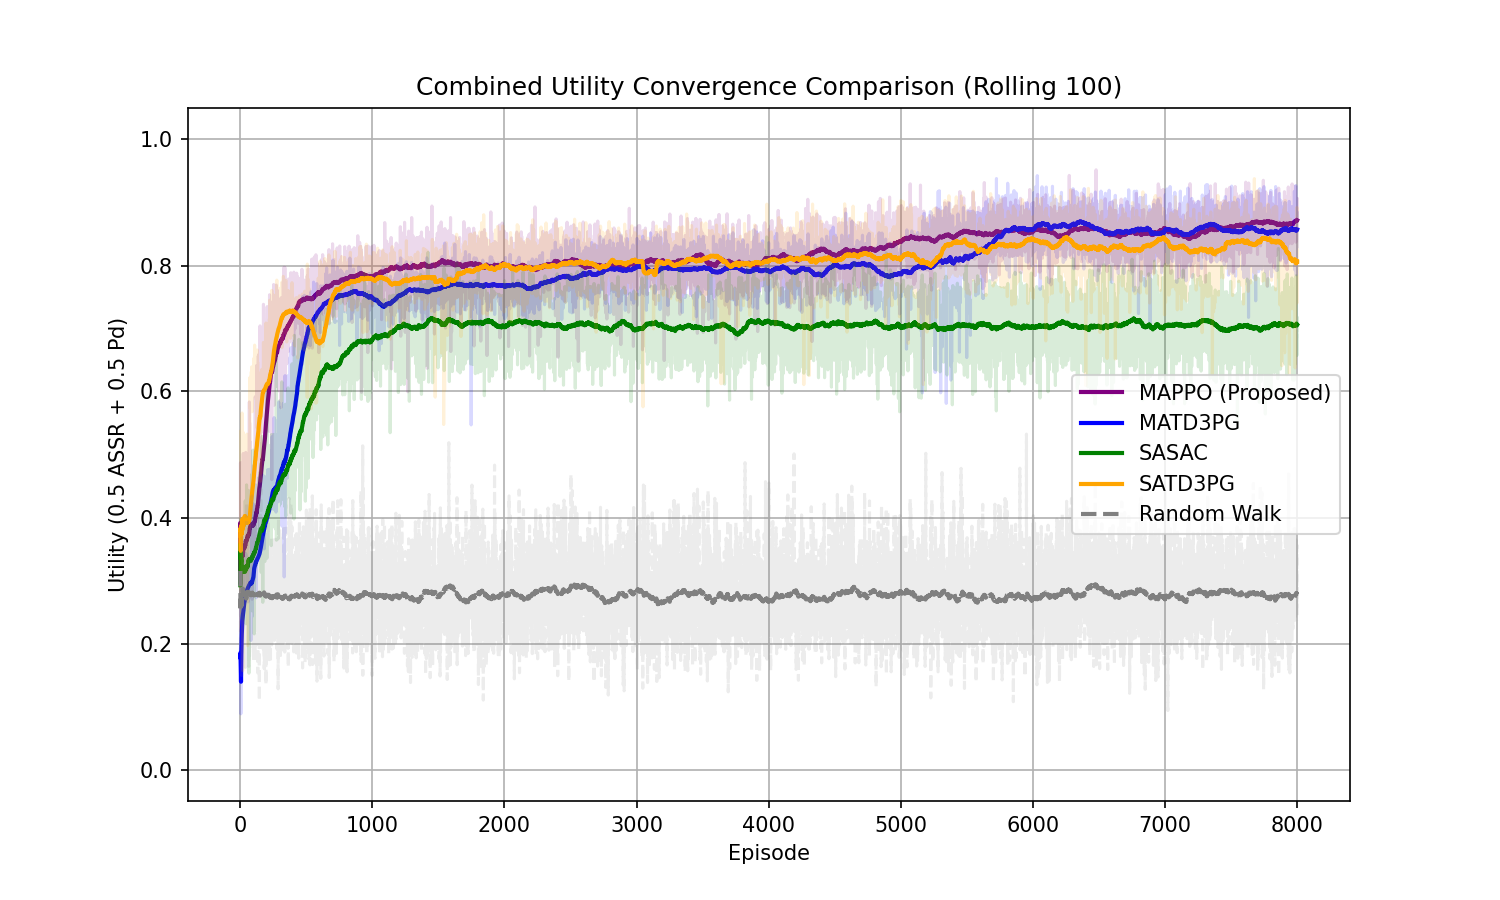
\includegraphics[width=0.65\textwidth]{convergence_comparison.png}
    \caption{Convergence comparison showing the rolling 100-episode average multi-objective utility $U = \lambda_1 \mathrm{ASSR} + \lambda_2 P_d$ for all four RL algorithms (MAPPO, MATD3PG, SASAC, and SATD3PG) and Random Walk.}
    \label{fig:convergence}
\end{figure}

\section{Conclusion and Future Directions}
In this updated report, we have presented a comprehensive mathematical framework for a semantic-aware ISAC network. Ground eavesdroppers are modeled with 3D location uncertainty bounded by a horizontal circle of radius $\Delta Q_e = 15.0\text{ m}$. We formulated the worst-case cascaded wiretap channels and generalized secrecy rate equations for $K_e$ eavesdroppers. Furthermore, we detailed the digital beamforming at the BS, passive analog phase-shift beamforming at the RIS, and multi-antenna digital jamming beamforming at the UAV Jammer. The DeepSC semantic metrics were modeled using a lookup table based on empirical evaluations ($M=10, K=15$). The performance of five reinforcement learning paradigms was analyzed under a combined utility objective. Future work will investigate joint dynamic trajectory planning and phase-shift optimization under time-varying fading channels.

\bibliographystyle{IEEEtran}

\end{document}
